% !TEX TS-program = XeLaTeX
% use the following command: 
% $ xelatex -shell-escape -output-driver="xdvipdfmx -z 0" article.tex
% this "-z 0" must be used to suppress compression in XMP Metadata packet 
% all document files must be coded in UTF-8
\documentclass{textolivre}
% for anonymous submission
%\documentclass[anonymous]{textolivre}
% to create HTML use 
%\documentclass{textolivre-html}
% remove all auxiliary files
% find . -name 'tl-article-template.*' ! -name '*.tex' ! -name '*.pdf' ! -name '*.bib' -type f -exec rm {} \;
% HTML compile using make4ht
% $ make4ht -c textolivre-html.cfg -u -x article "fn-in,svg"   # or use `mathjax' instead of `svg' to get LaTeX equation that will be handled by MathJax
% $ bibtex article
% clean and prettify HTML 
% $ tidy -o article-tidy.html --output-xhtml --break-before-br --wrap 0 article.html 2> errs.txt
% https://www.html-tidy.org/documentation/

% Metadata
\begin{filecontents*}[overwrite]{article.xmpdata}
    \Title{Concepções de letramento para o ensino da língua portuguesa em tempos de uso de artefatos digitais}
    \Author{Márcia Aparecida Vergna}
    \Language{pt-BR}
    \Keywords{Letramento \sep Multiletramentos \sep Novos estudos do letramento \sep Novos letramentos}
    \Journaltitle{Texto Livre}
    \Journalnumber{1983-3652}
    \Volume{14}
    \Issue{1}
    \Firstpage{1}
    \Lastpage{16}
    \Doi{10.35699/1983-3652.2021.24366}

    \setRGBcolorprofile{sRGB_IEC61966-2-1_black_scaled.icc}
            {sRGB_IEC61966-2-1_black_scaled}
            {sRGB IEC61966 v2.1 with black scaling}
            {http://www.color.org}
\end{filecontents*}

% PDF/A
% it is necessary to convert all image files to PDF/A
% use ghostscript as shown below:
% gs -dPDFA -dBATCH -dNOPAUSE -sColorConversionStrategy=UseDeviceIndependentColor -dCompatibilityLevel=1.4 -sDEVICE=pdfwrite -sProcessColorModel=DeviceCMYK -dPDFACompatibilityPolicy=2 -sOutputFile=image-a.pdf image.pdf

\journalname{Texto Livre: Linguagem e Tecnologia}
\thevolume{14}
\thenumber{1}
\theyear{2021}
\receiveddate{\DTMdisplaydate{2020}{07}{29}{-1}} % YYYY MM DD
\accepteddate{\DTMdisplaydate{2020}{09}{11}{-1}}
\publisheddate{\DTMdisplaydate{2020}{11}{07}{-1}}
% Corresponding author
\corrauthor{Márcia Vergna}
% DOI
\articledoi{10.35699/1983-3652.2021.24366}
% Abbreviated author list for the running footer
\runningauthor{Vergna, M.}

\title{Concepções de letramento para o ensino da língua portuguesa em tempos de uso de artefatos digitais}
\othertitle{Conceptions of literacy to the teaching of the portuguese language in times of use of digital artifacts}
% if there is a third language title, add here:
%\othertitle{Artikelvorlage zur Einreichung beim Texto Livre Journal}

\author[1]{Márcia Aparecida Vergna \thanks{Email: \url{marciavergna@yahoo.com.br}}}
\affil[1]{Universidade Estácio de Sá, Brasil.}

%\usepackage[backend=biber,style=abnt, ittitles]{biblatex}
%\DeclareLanguageMapping{brazil}{brazil-apa}
\addbibresource{article.bib}     
% use biber instead of bibtex
% $ biber tl-article-template
% $ pdflatex tl-article-template.tex

% set language of the article
\setdefaultlanguage[variant=brazilian]{portuguese}
\setotherlanguage{english}

\begin{document}
\maketitle

\begin{polyabstract}
\begin{abstract}
Este artigo objetiva apresentar um estudo teórico acerca das principais
concepções de letramento que embasam o ensino da Língua Portuguesa na
contemporaneidade. Para isso, desenvolvemos uma pesquisa bibliográfica. Na
atualidade, há, majoritariamente, três concepções teóricas acerca do
letramento: Novos Estudos do Letramento, Pedagogia dos Multiletramentos e Novos
letramentos, cujos principais representantes são Brian Street, Magda Soares e
Ângela Kleiman, para Novos Estudos do Letramento; Bill Cope, Mary Kalantzis e
Roxane Rojo, para Multiletramentos; e Colin Lankshear e Michele Knobel, para
Novos Letramentos. Depreende-se, do estudo, que toda visão de letramento está
atrelada a uma concepção de linguagem e a uma concepção de sociedade, e que a
escola é a principal agência desse letramento, tendendo a desenvolver suas
práticas de leitura e escrita a partir de um determinado posicionamento
ideológico, estabelecido por valores, relações de poder e perspectivas que
refletem o modelo de letramento escolhido para orientar a elaboração do
currículo a ser implementado e todo o trabalho em sala de aula.

\keywords{Letramento \sep Multiletramentos \sep Novos estudos do letramento \sep Novos letramentos}
\end{abstract}

\begin{english}
\begin{abstract}
This article aims to present a theoretical study about the main literacy
concepts that underlie the teaching of the Portuguese language in contemporary
times. For this, we developed a bibliographic research. Currently, there are
mostly three theoretical conceptions about literacy: New Literacy Studies,
Pedagogy of Multiliteracies and New Literacies, whose main representatives are
Brian Street, Magda Soares and Ângela Kleiman, for New Literacy Studies; Bill
Cope, Mary Kalantzis and Roxane Rojo, for Multi-tools; and Colin Lankshear and
Michele Knobel, for New Literacies. It appears from the study that every
literacy view is linked to a conception of language and to a conception of
society, and that the school is the main agency of this literacy, tending to
develop its reading and writing practices from a certain ideological
positioning, established by values, power relations and perspectives that
reflect the literacy model chosen to guide the elaboration of the curriculum to
be implemented and all the work in the classroom.

\keywords{Literacy \sep Multiliteracies \sep New literacies \sep New literacy studies}
\end{abstract}
\end{english}

% if there is another abstract, insert it here using the same scheme
\end{polyabstract}


\section{Introdução}\label{sec-intro}
De acordo com \textcite{soares2017}, em meados dos anos 1980, tanto no Brasil quanto em
outros países, já não era suficiente apenas saber ler e escrever, ou seja,
codificar e decodificar, era necessário que as práticas de leitura e escrita
fossem além das práticas do ler e do escrever, resultando, assim, no surgimento
do termo letramento para nomear comportamentos e práticas sociais na área da
leitura e da escrita que ultrapassassem o domínio do sistema alfabético e
ortográfico.

Essa necessidade se deu em função de a vida social e as atividades
profissionais terem se tornado cada vez mais centradas na e dependentes da
língua escrita, sendo insuficiente, para esse novo contexto, apenas alfabetizar
a criança ou o adulto. No Brasil, a palavra letramento surgiu no campo da
Educação e das Ciências Linguísticas, mais especificamente no ano de 1986, com
a publicação do livro intitulado \citetitle*{kato1986} de 
%Mary Kato
%\theauthorname{kato1986}
\citefirstlastauthor{kato1986} 
\cite{soares2017}.
%\textit{No mundo da escrita: uma perspectiva psicolinguística}, de Mary Kato (SOARES, 2017).

Vários pesquisadores têm se dedicado ao estudo do letramento, suscitando também
diferentes visões acerca de sua concepção. Tal concepção de letramento sofreu
ressignificações ao longo do tempo, mostrando-se complexo e dinâmico, sendo
interpretado e definido de vários modos, e influenciado por diversos fatores
que trazem enraizados valores culturais e experiências pessoais. Estudos
históricos, antropológicos e etnográficos revelam que houve mudanças na
concepção de letramento ao longo do tempo, dependendo das crenças, valores e
práticas culturais de cada grupo social \cite{soares2004}.

Ao construir concepções, o ser humano constrói também valores, que implicam
posicionamentos que se materializam em dizeres. Essa compreensão se aproxima do
viés bakhtiniano, por defender que todo ser humano é atravessado por múltiplas
vozes sociais, e que vai se constituindo socialmente, por meio de saberes e
conhecimentos com que tem contato, na relação intersubjetiva que estabelece com
outros seres sociais em diferentes campos de atuação.

Nessa perspectiva, este artigo objetiva apresentar um estudo teórico acerca de
algumas concepções de letramento que embasam o ensino da Língua Portuguesa no
Brasil.



\section{Surgimento do termo letramento no Brasil}\label{sec-surgimento}
\textcite[p. 35]{soares2004}, uma das pioneiras a estudar
a temática no país, afirma que o termo letramento foi introduzido na língua
portuguesa, originando-se da palavra da língua inglesa \textit{literacy}, que tem como
conceito “’\textit{the condition of being literate}’, ou seja, a condição de ser letrado
[...].” Literate é definido como sendo “\textit{educated; especially able to read and
write}” \cite[p. 35]{soares2004}. Letrado, nesse sentido, significa a pessoa que
domina a leitura e a escrita. Assim, “[...] \textit{literacy} designa o estado ou
condição daquele que é literate, daquele que não só sabe ler e escrever, mas
também faz uso competente e frequente da leitura e da escrita” \textcite[p. 36]{soares2004}.
Para a autora, o surgimento do termo se deu em função de que
\begin{quote}
Antes, nosso problema era apenas o do 'estado ou condição de analfabeto' – a
enorme dimensão desse problema não nos permitia perceber esta outra realidade,
o “estado ou condição de quem sabe ler e escrever”, e, por isso, o termo
analfabetismo nos bastava, o seu oposto – alfabetismo ou letramento – não nos
era necessário, porque só recentemente passamos a enfrentar esta nova realidade
social em que não basta apenas saber ler e escrever, é preciso também saber
fazer uso do ler e do escrever, saber responder às exigências de leitura e de
escrita que a sociedade faz continuamente – daí o recente surgimento do termo
letramento \cite[p. 20]{soares2004}.
\end{quote}

Assim, num primeiro momento, as habilidades de leitura e escrita estiveram
ligadas ao conceito de alfabetização, surgindo, posteriormente, novas demandas
no campo das práticas de leitura e escrita e, para designá-las, utilizou-se o
termo letramento. Essas novas demandas referem-se à preocupação que os estudos
linguísticos passaram a ter, no Brasil, a partir da década de 1980, com o uso
social da leitura e da escrita. Preocupação essa advinda, em parte, dos estudos
de \textcite[p. 9]{freire1989}, o qual afirmou que “a leitura do mundo precede a
leitura da palavra, daí que a posterior leitura desta não possa prescindir da
continuidade da leitura daquele”.

O autor propôs uma compreensão mais crítica da leitura, que fosse além da
decodificação da escrita, ampliando seu conceito para a compreensão do mundo,
utilizando alfabetização, ao que nos parece, no sentido de letramento. Nesse
sentido, \textcite{freire1989} é quem aparenta inaugurar a concepção de letramento, tal
qual estamos aqui considerando:
\begin{quote}
Inicialmente, me parece interessante reafirmar que sempre vi a alfabetização de
adultos como um ato político e um ato de conhecimento, por isso mesmo, como um
ato criador. Para mim seria impossível engajar-me num trabalho de memorização
mecânica dos ba-be-bi-bo-bu, dos la-le-li-lo-lu. Daí que também não pudesse
reduzir a alfabetização ao ensino puro de palavras, de sílabas ou das letras
\cite[p. 13]{freire1989}.
\end{quote}

\textcite{freire1989} utiliza apenas o termo alfabetização para abarcar esses processos.

\textcite[. 47]{soares2004} define letramento como sendo o “estado ou condição
de quem não apenas sabe ler e escrever, mas cultiva e exerce as práticas
sociais que usam a escrita”. Emerge, assim, uma diferença entre alfabetização e
letramento. Enquanto este é compreendido no contexto das práticas sociais, como
consequência de ter se apropriado da alfabetização, aquela é compreendida como
apenas codificação/decodificação.

A diferença entre alfabetização e letramento também fica bem evidente na
definição de \textcite[p. 19]{kleiman2003}, que considera que letramento é “um conjunto
de práticas sociais que usam a escrita, enquanto sistema simbólico e enquanto
tecnologia, em contextos específicos, para objetivos específicos”. Nesse
sentido, as habilidades requeridas para as práticas de leitura e escrita, os
valores ideológicos vinculados a essas habilidades e os efeitos sociais e
cognitivos derivados do uso da leitura e escrita variam em diferentes culturas,
contextos institucionais e períodos históricos.

Assim, enquanto a alfabetização é um processo de aquisição de códigos, o
letramento é um processo muito mais amplo, em que a escrita, a compreensão e a
interação estão imbricadas. Nessa concepção, o conceito de letramento liga-se
às práticas sociais de leitura e de escrita. Contudo, vale ressaltar que,
inicialmente, o letramento era concebido como uma prática individual, sendo um
conjunto de habilidades cognitivas ou psicológicas que as pessoas possuíam, e
que poderiam ser ensinadas de maneira neutra em contextos formais ou informais
de ensino. Essa era a visão tradicional de letramento, dominante até então.



\section{Principais concepções de letramento}\label{sec-principais}
\subsection{Novos Estudos do Letramento}\label{sec-novos-estudos}
A partir do século XX, um grupo de estudiosos anglo-saxões passou a desenvolver
estudos que focavam muito mais o lado social do letramento do que seu lado
cognitivo. Os estudos buscavam compreender o impacto sociocognitivo e cultural
da escrita, bem como as práticas de letramento, sendo denominado Novos Estudos
do Letramento (NEL).

A palavra “novo” se refere basicamente a uma mudança de paradigma, que retira
de foco a mente do indivíduo, e passa a considerar leitura e escrita a partir
do contexto das práticas sociais e culturais. “Anteriormente, o foco de boa
parte da pesquisa acadêmica incidia sobre consequências cognitivas da aquisição
de letramento” \cite[p. 17]{street2014}.

Na concepção de teóricos dos Novos Estudos do Letramento ou teoria social do
letramento, que tem como principal representante o antropólogo britânico Brian
Vincent Street, a escrita tem um caráter social. Assim, o termo letramento
refere-se a todas as práticas sociais que envolvem a leitura e a escrita em
determinada sociedade, sendo variáveis de um grupo social para outro \cite{street2014}.
Nessa concepção, rejeita-se a visão dominante do letramento como uma
habilidade “neutra”, técnica, passando a percebê-lo como uma prática
ideológica, envolvida em relações de poder e incrustada em significados e
práticas culturais específicos \cite{street2014}.

Nessa concepção, pessoas não alfabetizadas, isto é, que não dominam o código
escrito, também são consideradas letradas, desde que participem de práticas
sociais que, direta ou indiretamente, envolvam a escrita. O foco dos Novos
Estudos do Letramento não está no domínio do código, mas na manipulação dele ou
mesmo na relação que os indivíduos mantêm com ele, ainda que não o dominem,
como quando, por exemplo, um sujeito analfabeto participa do momento da leitura
da bíblia em uma cerimônia religiosa.

Os adeptos dessa concepção buscaram evidenciar que todas as práticas de
letramento são consequências da cultura e das estruturas de poder da sociedade
da qual a pessoa faz parte. Por isso, elas se modificam ou se transformam
segundo o contexto em que se desenvolvem.

\textcite{street2014}, a partir de suas pesquisas, definiu dois modelos de letramento:
o autônomo e o ideológico.

O modelo de letramento autônomo concebe a escrita como um instrumento ou
tecnologia que independe do contexto social no qual a pessoa está inserida, e é
associada ao progresso, à civilização, à liberdade individual e à mobilidade
social. Está embasado em uma abordagem universal, neutra, independente da
cultura, baseado em habilidades cognitivas, e impõe concepções particulares a
outras classes sociais, grupos e culturas \cite{street2014}. Esse modelo concebe a
escrita como um ato individual, independente de suas condições sociais, sendo
concebida como um
\begin{quote}
um produto completo em si mesmo, que não estaria preso ao contexto de sua
produção para ser interpretado; o processo de interpretação estaria determinado
pelo funcionamento lógico interno ao texto escrito, não dependendo das (nem
refletindo, portanto) reformulações estratégicas que caracterizam a oralidade,
pois, nela, em função do interlocutor [...]. Assim, a escrita representaria uma
ordem diferente de comunicação, distinta da oral, pois a interpretação desta
última estaria ligada à função interpessoal da linguagem, às identidades e
relações que interlocutores constroem, e reconstroem, durante a interação
\cite[p. 22]{kleiman2003}.
\end{quote}

Nesse modelo estabelecem-se os conhecimentos que devem ser transmitidos, uma
vez que é essa transmissão a produtora de efeitos sobre capacidades cognitivas.
Assim, ao serem expostos a um mesmo tipo de letramento padronizado, diferentes
grupos desenvolverão as habilidades cognitivas desejáveis. A partir delas, se
desenvolverão competências e habilidades relativas à leitura e escrita, que, em
tese, propiciarão aos cidadãos o acesso ao trabalho, à informação e à
cidadania, independentemente das reais condições em que vivem. Dessa forma, o
letramento é reduzido a um conjunto de capacidades cognitivas que podem ser
medidas nos sujeitos, daí resultando em expressões como “grau de letramento”,
“nível de letramento” ou “baixo letramento”.

Nessa concepção, \textcite{street2014} afirma que as políticas públicas nacionais e
internacionais de avaliação da compreensão leitora dos alunos ao término do
Ensino Fundamental e do Ensino Médio, os concursos públicos, o ENEM são bons
exemplos de ações sociais que revelam e legitimam essa concepção autônoma,
centrada no sujeito e nas capacidades de usar apenas o texto escrito. Para
\textcite[p. 9]{street2014}, “[...] o foco central está na análise das capacidades
cognitivas individuais”. Assim, “no que diz respeito ao letramento
escolarizado, é evidente que, em geral, o modelo autônomo de letramento vem
dominando o currículo e a pedagogia \cite[p. 150]{street2009}.

Já o modelo ideológico parte da premissa de “[...] que o letramento é uma
prática social, e não simplesmente uma habilidade técnica e neutra [...]”
\textcite[p. 53]{street2014}. Envolve também aspectos relacionados à cultura e à
história de determinado grupo social; portanto, é mais do que a habilidade de
grafar e/ou decodificar letras. O termo ideológico “[...] indica bem
explicitamente que as práticas letradas são aspectos não só da ’cultura’ como
também das estruturas de poder” \cite[p. 172]{street2014}.

Nesse modelo, os alunos não só compreendem os textos que leem, mas também
conseguem utilizar a escrita de forma satisfatória à situação social
apresentada. O letramento é vinculado às forças ideológicas e políticas que
constituem as instituições sociais das quais ele faz parte, ou seja, o
significado das práticas de leitura e escrita é construído nas interações que
ocorrem dentro de estruturas sociais específicas, uma vez que
\begin{quote}
[...] não tenta negar a habilidade técnica ou os aspectos cognitivos da leitura
e da escrita, mas sim entendê-los como encapsulados em todos culturais e em
estruturas de poder. Nesse sentido, o modelo ideológico subsume, mais do que
exclui, o trabalho empreendido dentro do modelo autônomo \cite[p. 172]{street2014}.
\end{quote}

Esse modelo parece se aproximar do conceito freireano de alfabetização, embora
\textcite{street2014} não tenha se referido a esse campo conceitual.

De acordo com \textcite{street2014}, aqui no Brasil, os modelos autônomo e
ideológico, discutidos por ele ainda em 1984, foram mobilizados e apresentados
por Ângela Kleiman em 1995 em uma coletânea que teve o objetivo de discutir os
“significados do letramento” e “uma nova perspectiva sobre a prática social da
escrita”.

Outra questão central, para compreendermos o letramento como um fenômeno social, 
proposta pelos teóricos dos Novos Estudos do Letramento, refere-se a eventos de
letramento e práticas de letramento.

Eventos de letramento correspondem a qualquer ocasião em que um fragmento de
escrita integra a natureza das interações dos participantes e seus processos
interpretativos \cite{street2014}. São, em geral, atividades que utilizam textos
escritos para serem lidos ou para se falar sobre eles; episódios observáveis
que emergem de práticas e são por elas moldados, mediados por textos escritos.
Os eventos de letramento identificam a ocorrência de uma situação social na
qual a escrita assume um papel central, ou seja, são as ocasiões em que a
escrita medeia a interação.

De acordo com \textcite{street2014}, as palestras representam um clássico
exemplo do conceito de eventos de letramento: o palestrante pode ler suas
anotações; um projetor de slides com diferentes tipos de informações; as
pessoas podem olhar para a projeção no alto, baixar o olhar e fazer uma
anotação, ler sua anotação e voltar a escutar o palestrante. Portanto, há
“[...] uma mescla de traços orais e letrados na comunicação cotidiana” \textcite[p. 146]{street2014},
havendo, portanto, um diálogo entre os participantes, mesmo que
estes estejam ausentes ou sejam imagináveis. \textcite[p. 25]{barton2015} afirmam
que “o essencial nos eventos de letramento é a interação da escrita e da fala,
pois um evento de letramento pode ter fala em torno de um texto.”

Já as práticas de letramento dizem respeito aos “modos culturais de utilização
da escrita”, correspondendo às relações sociais que se estabelecem em torno dos
usos escritos, às valorações que a modalidade escrita recebe nas diversas
vivências. “O conceito de práticas de letramento se coloca num nível mais alto
de abstração e se refere igualmente ao comportamento e às conceitualizações
sociais e culturais que conferem sentido aos usos da leitura e/ou da escrita”
\cite[p. 18]{street2014}.

\textcite{barton2015} afirmam que quando uma pessoa comenta uma notícia
on-line, reserva um ingresso, joga ou marca um encontro com um amigo está
negociando a língua escrita, ocorrendo eventos de letramento, e ao decidir onde
e quando fazer essas coisas, juntamente com quais estilos de linguagem usar, os
participantes empregam suas práticas de letramento.

Os autores ainda afirmam que, em um planejamento de um feriado, prática social
reconhecível, a checagem dos horários do voo e a reserva de bilhetes podem ser
vistas como práticas de letramento, pois há padrões comuns na utilização da
leitura e escrita no contexto do planejamento do feriado. “Práticas de
letramento são constituídas por atividades específicas e, ao mesmo tempo, fazem
parte de processos sociais mais amplos [...]” \cite[p. 40]{barton2015}.
Eventos de letramento são as ocasiões em que o texto escrito figura como
central, enquanto as práticas de letramento dizem respeito às crenças,
concepções e valores atribuídos à leitura e à escrita em determinado contexto,
ou seja, eventos correspondem à parte visível e práticas à parte invisível do
letramento.

Nesse contexto, \textcite{street2014} pontua que no modelo ideológico a variedade de
práticas de leitura e escrita que integram o letramento permite considerá-lo
algo plural, ou seja, é possível falar em letramentos e não em um único
letramento. \textcite[p. 53]{terra2020} esclarece que a “[...] a constituição de
diferentes tipos de letramento está intrinsecamente ligada à inserção do
indivíduo em determinadas esferas da atividade humana (família, escola,
trabalho, igreja etc.) nas quais circulam uma infinidade de textos/gêneros
escritos”. Nessa perspectiva, o professor de Língua Portuguesa deve pautar seu
trabalho a partir de práticas situadas, dos gêneros do cotidiano do aluno,
como, por exemplo, os que circulam na esfera doméstica: bilhetes, lista de
compras, dentre outros, desenvolvendo situações de uso real da linguagem, e não
apenas privilegiando, na sala de aula, os textos dos letramentos dominantes da
sociedade.

A concepção dos Novos Estudos do Letramento está mais intimamente ligada aos
textos escritos. \textcite[p. 3]{bragana2016} explicam que “o termo
‘letramento’, dentro dos Novos Estudos do Letramento (NEL), reporta-se a todos
os usos sociais da escrita; dito de outra forma, ao conjunto de práticas
sociais mediadas pela escrita, direta ou indiretamente”. Para \textcite[p. 91]{street2009},
as áreas do conhecimento é que determinam os vários gêneros de escrita, de
acordo com “o tema, o período do aluno, dentre outros fatores”. Porém, com o
advento e disseminação do uso das tecnologias de informação e comunicação,
surgiu a necessidade de considerar os textos que vão além das concepções
tradicionais de ensino pautadas em uma visão estática e monomodal da linguagem.
Segundo \textcite[p. 81]{kleiman2014},
\begin{quote}
[...] o texto digital, com suas combinatórias de diversas linguagens com modos
específicos de significar; a constatação do aumento progressivo da presença da
imagem no texto em que antes predominava a linguagem verbal; e o interesse em
estudar essas mutantes formas de comunicação definiram, em 1996, para o chamado
“New London Group (Grupo de Nova Londres), um novo objeto de estudo, os
multiletramentos”.
\end{quote}

Essa concepção de letramento será abordada na seção seguinte.

\section{Pedagogia dos Multiletramentos}\label{sec-pedagogia}
Apesar da relevância do letramento voltado para a linguagem verbal, surge a
necessidade de pensar novas formas de letramento\footnote{
As reuniões começaram em 1994 para conversar sobre o que estava acontecendo no
mundo das comunicações e no ensino, haja vista as transformações por que estava
passando a humanidade \cite{cope2009}.
}. Um grupo de pesquisadores, o Grupo de Nova Londres\footnote{
O Grupo é composto por Courtney Cazden, Bill Cope, Charles William Eliot, Jim
Gee, Norman Fairclough, Mary Kalantzis, Allan Luke, Carmen Luke, Martin Nakata
e Sara Michaels \cite{cope2009}.
}, apontou o termo multiletramentos para definir uma nova abordagem, a qual
oferece argumentos para repensar os letramentos e suas implicações para a
participação social na vida pública, econômica e comunitária \cite{cope2009}.
Os pesquisadores publicaram, em 1996, “[...] um manifesto intitulado A Pedagogy
of Multiliteracies – Designing\footnote{A palavra 'design' descreve os padrões
significado e ação que constituem representação, comunicação e interpretação
\cite{cope2009}.} Social Futures (Uma Pedagogia dos
Multiletramentos – desenhando futuros sociais) \cite[p. 12]{rojo2012}, resultante
de um colóquio realizado em Nova Londres, Estados Unidos.

O manifesto chamava a atenção para a necessidade de a escola se apropriar dos
novos letramentos emergentes na sociedade e de considerar as diferenças
culturais presentes nas salas de aula, haja vista a multiplicidade de canais de
comunicação e a diversidade linguística e cultural presentes no mundo. Assim, o
termo multiletramentos aponta para dois aspectos: multiplicidade semiótica de
constituição dos textos e multiplicidade de culturas \cite{rojo2012}.

A multiplicidade semiótica refere-se à multiplicidade de linguagens, ou seja,
textos compostos de muitas linguagens, denominada modos ou semioses, como o
linguístico, o visual, o auditivo, o gestual e o espacial, por exemplo \cite{cope2009}.

A multiplicidade de culturas, de acordo com \textcite{rojo2012}, refere-se às produções
culturais letradas que circulam na sociedade, como um conjunto de textos
híbridos de diferentes letramentos (vernaculares e dominantes) e de diferentes
campos (popular, de massa, erudito). A autora esclarece que o Grupo de Nova
Londres considera necessário, por exemplo, desenvolver habilidades referentes a
negociar dialetos regionais, étnicos ou baseados em classes; variações no
registro que ocorrem de acordo com o contexto social e discursos transculturais
híbridos, por exemplo.

Na concepção dos Multiletramentos, propõe-se formar um usuário funcional, que
tenha competência técnica, que entenda como diferentes tipos de texto e
tecnologia operam, que tenha criticidade e que seja capaz de promover
transformações \cite{rojo2012}. O diagrama abaixo evidencia esses princípios.

\begin{figure}[htbp]
 \centering
 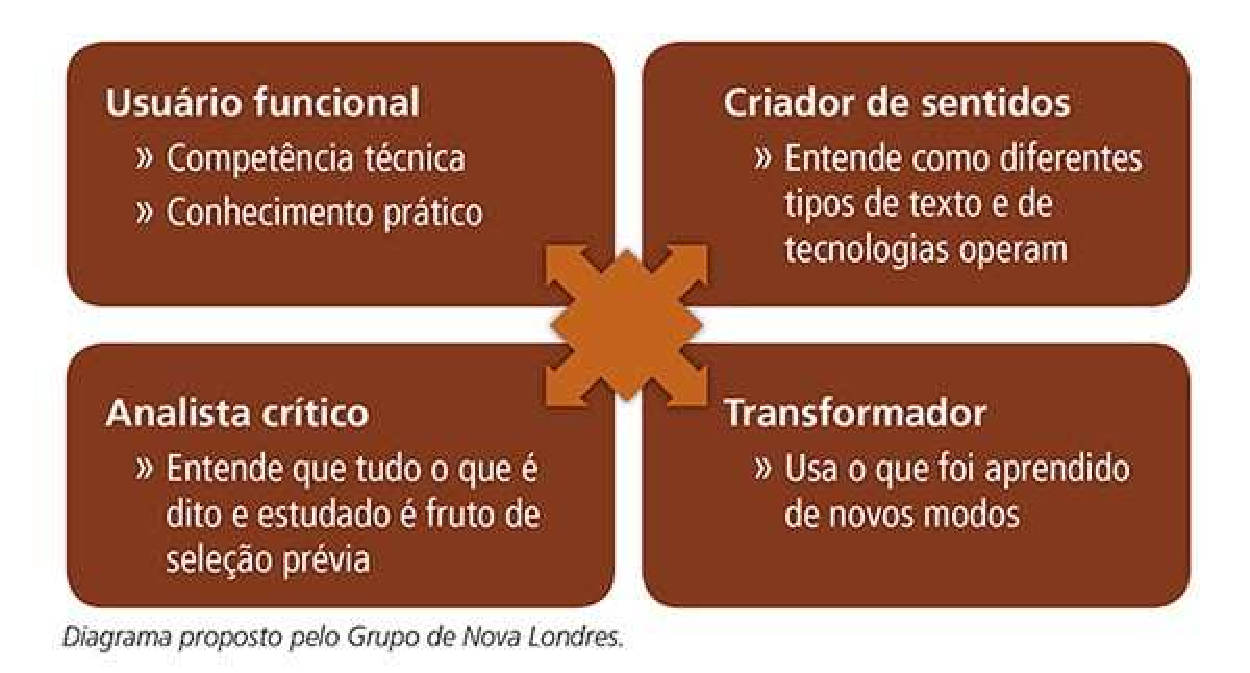
\includegraphics[width=0.5\textwidth]{figure01.pdf}
 \caption{Prática na Pedagogia dos Multiletramentos.}
 \label{fig01}
 \source{adaptado de \textcite{cope2009}.}
\end{figure}

O Grupo de Nova Londres considera que a mente humana é incorporada, situada e
social, ou seja, o conhecimento humano está embutido em contextos sociais,
culturais e materiais e seu conhecimento desenvolvido como parte de um processo
de interações colaborativas com outros de diferentes habilidades, contextos e
perspectivas que fazem parte de uma mesma comunidade \cite{cope2009}, o
que leva os autores a propor uma pedagogia como uma complexa integração de
quatro fatores, não necessariamente em uma sequência fixa: 
\begin{enumerate*}[label=\alph*)]
\item prática situada;
\item instrução aberta;
\item enquadramento crítico;
\item prática transformada. 
\end{enumerate*}

\textcite{rojo2012} esclarece que \emph{prática} situada refere-se à imersão do aluno
na experiência e utilização de projetos disponíveis – mundo do aluno e
simulações dos relacionamentos encontrados nos locais de trabalho e nos espaços
públicos, ou seja, práticas que fazem parte da cultura dos alunos e nos gêneros
e \emph{designs} disponíveis para essa prática, relacionando-as com outras, de outros
espaços culturais. \emph{Instrução aberta} consiste em os aprendizes moldarem para si
mesmos uma metalinguagem explícita do design. \emph{Enquadramento crítico} consiste em
relacionar os sentidos aos seus contextos e propósitos sociais. \emph{Prática
transformada} se dá quando os aprendizes transferem e recriam designs de
sentidos de um contexto para o outro.

Em 2006, tendo em vista as transformações que ocorreram na humanidade desde
1996, quando da publicação do Manifesto, \textcite{cope2009} reformularam esses
componentes traduzindo-os em “processos de aprendizagem”, ou, ainda,
orientações pedagógicas, passando a denominá-los experienciando,
conceitualizando, analisando e aplicando, conforme \Cref{tbl01}.

\begin{table}[htbp]
\caption{Processos de Aprendizagem.}
\label{tbl01}
{ \small
\begin{tabular}{p{0.47\textwidth} p{0.47\textwidth}}
\headrow \thead{Orientações pedagógicas – formulação de 1996} & \thead{Processos de conhecimento – reformulação de 2006} \\
Prática situada & Experienciando \newline ... o conhecido \newline ... o novo \\
Instrução aberta & Conceitualizando \newline ... por nome \newline ... com teoria \\
Enquadramento crítico & Analisando \newline ... funcionalmente \newline ... criticamente \\
Prática transformada & Aplicando \newline ... apropriadamente \newline ... criativamente
\end{tabular}
}
\source{\textcite[p. 26, tradução nossa]{cope2009}.}
\end{table}


\textcite{cope2009} afirmam que experienciando consiste em levar o aluno a
refletir sobre suas próprias experiências, interesses, ou seja, aquilo que lhe
é conhecido, bem como o experienciamento do novo, permitindo-lhe entrar em
contato com novas situações, levando-os a novos domínios de ação e significado.
Faz-se a valorização dos conhecimentos extraescolares dos alunos,
permitindo-lhes relacionar saberes prévios e novas informações e experiências,
ocorrendo, dessa forma, o entrelaçamento do novo com o conhecido.

\emph{Conceitualizando} refere-se a definir e aplicar conceitos.
“Conceitualizando por nome envolve distinções de similaridades e diferenças,
categorias e nomes abstratos. Conceitualizando com teoria significa fazer
generalizações e construir modelos que possam ser transferidos” \cite[p. 31]{raulik2916}. 
Assim, \emph{conceitualizando} refere-se ao entrelaçamento entre conhecimento
que adquirimos no dia a dia e o conhecimento científico. \textcite[p. 14]{silva2016}
esclarece que “é a partir da junção de diversos conceitos que o conhecimento da
disciplina é construído como um todo”.

\emph{Analisando} refere-se à capacidade crítica em que se busca estabelecer
raciocínios a fim de extrair inferências, conclusões, estabelecendo relação de
causa e efeito e da razão de ser das coisas, evidenciando os objetivos,
motivos, intenções e pontos de vista das pessoas. “Analisando funcionalmente
inclui analisar processos de causa e efeito, analisar conexões lógicas e
textuais, desenvolver cadeias de raciocínio e explicar padrões. Analisando
criticamente envolve a avaliação das perspectivas, interesses e motivações das
pessoas” \cite[p. 31]{raulik2916}. \emph{Analisando} envolve, portanto, a capacidade de
os alunos questionarem, por exemplo, os interesses implícitos em uma mensagem
ou ação.

\emph{Aplicando} consiste em o aluno aplicar o conhecimento ao seu mundo real,
ou em situações que se aproximem do real, fazendo uma intervenção criativa, que
afete o mundo de maneira positiva, transferindo um conhecimento anterior para
um novo cenário. “Aplicando apropriadamente significa que o aluno fará algo de
maneira previsível e já esperada. Aplicando criativamente inclui uma
intervenção criativa e inovadora de acordo com os interesses, experiências e
aspirações do aluno” \cite[p. 31]{raulik2916}.

Esses componentes propõem um letramento diferente das concepções mais antigas
em que os alunos eram vistos como passivos e meros recipientes, cujo papel
consistia em memorizar e reproduzir o que recebiam do professor como verdade
única \cite{cope2009}, sendo necessário, nesse novo contexto, que os alunos
projetem significados àquilo que lhes é apresentado, sendo capazes de
participar de diversos letramentos, tanto no que se refere aos diferentes
contextos culturais e institucionais de uso da leitura e da escrita como na
escola, no trabalho, no lazer, nas atividades cívicas, quanto no que se refere
ao uso de diferentes códigos e linguagens, como, por exemplo, a escrita
alfabética, a representação visual, a comunicação gestual, a comunicação sonora
e musical, e diferentes mídias (por exemplo, o corpo, a escrita, a imprensa, a
mídia eletrônica – como rádio e televisão, as mídias digitais).

O Grupo de Nova Londres considera que lidar com as diferenças linguísticas e
culturais tornou-se ponto central para o mundo do trabalho, da cidadania e da
vida privada. Consideram que na Pedagogia dos Multiletramentos educadores e
estudantes podem se ver como participantes ativos da mudança social, pois podem
ser designers ativos, ou seja, criadores de futuros sociais, pensando na
questão da formação para o trabalho, para a cidadania, para a vida pessoal.

A ideia de design\footnote{
Observamos uma divergência quanto à tradução do termo para o português: alguns
trabalhos apontam design como “desenho”, outros como “projeto”.
} é um conceito chave para a Pedagogia dos Multiletramentos.
\textcite{cope2009} afirmam que essa palavra apresenta duplo significado:
descreve, simultaneamente, estrutura ou morfologia, e o ato de construção.
Afirmam que conhecimento e significado são situados histórica e socialmente, e
são projetados, sendo por isso, chamado de design. Este, conforme \Cref{tbl02},
apresenta três aspectos: \emph{designs disponíveis}, \emph{designing} e \emph{the redesigned}.

\begin{table}[htpb]
\caption{\emph{Designs}.}
\label{tbl02}
\begin{tabular}{lp{10cm}}
\toprule
Designs disponíveis & Recursos culturais e contextuais para a construção do sentido, incluindo modo (linguístico, visual, espacial, gestual, etc.), gênero e D/discurso. \\
\midrule
Designing & Processo de construção e recontextualização da representação do mundo por meio dos designs disponíveis. Ato de apropriação, de “revozeamento” dos designs disponíveis. \\
\midrule
The redesigned & Produto do ato de design sempre transformado e que, assim, constitui um novo design disponível. O mundo transformado em novos designs disponíveis, que instanciam novos sentidos. \\
\bottomrule
\end{tabular}
\source{\cite[p. 176, tradução nossa]{cope2009}.}
\end{table}


\textcite{cope2009} afirmam que designs disponíveis referem-se às formas
representacionais encontradas. Para eles, os padrões e convenções para
representação de significados podem ser constituído de modo (linguístico,
visual, áudio, gestual, tático e espacial), de gênero (a forma que um texto
possui) e de discurso (a forma que significa fazer tomadas em uma instituição
social). \emph{Designing} é o ato de apropriação, de “revozeamento” e de transformação
dos designs disponíveis; refere-se à apropriação dos projetos disponíveis para
fazer as representações do mundo ou de outros para si ou para os outros (como
escrever, falar, tirar fotos, ler, ouvir, visualizar, por exemplo). Com isso,
cria-se um novo design, uma expressão da voz do aluno. O \emph{redesigned} refere-se
às transformações ocasionadas nas pessoas e no mundo pelo ato de projetar. A
\Cref{fig02} ilustra os modos de significação dos \emph{designs} disponíveis.

\begin{figure}[htbp]
 \centering
 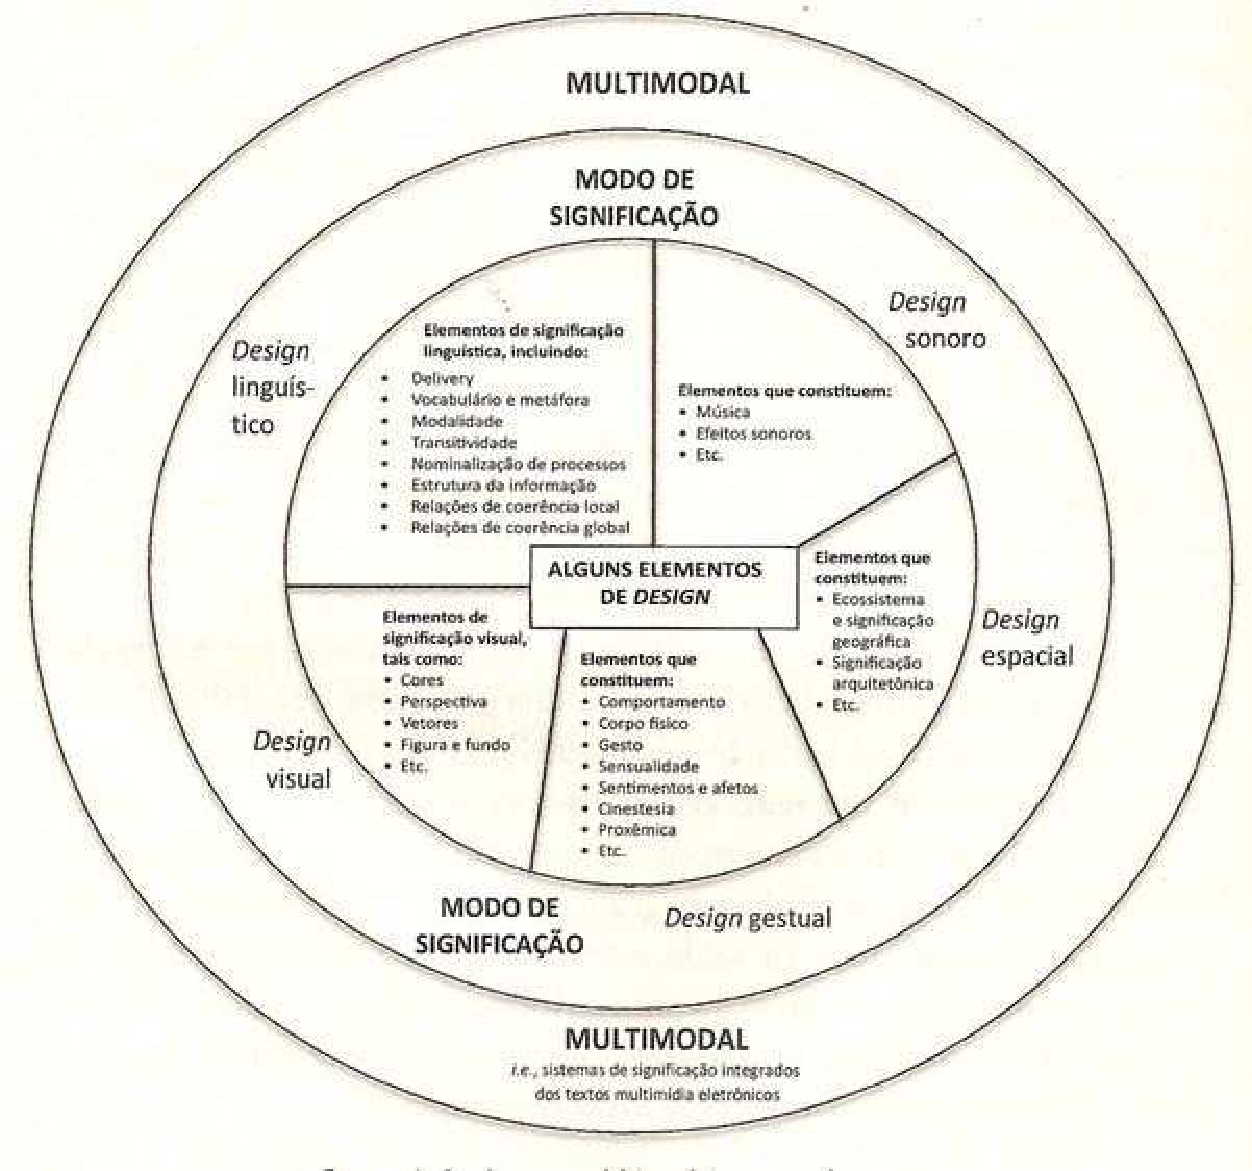
\includegraphics[width=0.75\textwidth]{figure02.pdf}
 \caption{Modos de significação dos designs disponíveis.}
 \label{fig02}
 \source{\apud[p. 26]{novalondres}[p. 24]{rojo2013}.}
\end{figure}

O \emph{design} multimodal é de ordem diferente dos outros cinco modos de
significado, pois representa os padrões de interconexão entre os outros modos.
Para o grupo,
\begin{quote}
[...] somos herdeiros de padrões e convenções de significado e, ao mesmo tempo,
designers ativos de significado. E, como designers de significado, somos
designers de futuros sociais – local de trabalho futuros, futuros públicos e
futuros da comunidade \cite[p. 65, tradução nossa]{cazden1996}\footnote{
“[...] we are both inheritors of pattern and conventions of meaning and at the
same time active designers of meaning. And, as designers of meaning, we are
designers of social futures – workplace futures, public futures, and community
futures” \cite[p. 65]{cazden1996}.
}. 
\end{quote}

De acordo com \textcite{cope2009}, o modelo proposto contempla as formas de
representar significados dos diferentes sistemas semióticos – linguístico,
visual, sonoro ou auditivo, espacial e gestual – inter-relacionados no texto
multimodal contemporâneo, estando, portanto, a linguagem inseparavelmente
relacionada a esses modos de significado.

Tendo em vista que muitas transformações aconteceram desde 1996, \textcite{cope2009}
reconfiguraram essa gama de modalidades possíveis: separaram a
linguagem escrita da oral, adicionaram um modo tátil e redefiniram o conteúdo e
o escopo dos outros modos. A \Cref{tbl03} mostra como ficou essa alteração:

\begin{table}[htpb]
\caption{Formas de representar significados dos diferentes sistemas semióticos.}
\label{tbl03}
\begin{tabular}{lp{8cm}}
\toprule
Linguagem escrita & Escrita (representando significado para o outro) e leitura (representando significado para si mesmo) – caligrafia, página impressa, tela. \\
\midrule
Linguagem oral & Fala ao vivo ou gravada (representando significado para o outro); ouvir (representando significado para si mesmo). \\
\midrule 
Representação visual & Imagem estática ou em movimento, escultura, artesanato (representando significado para o outro); vista, cena, perspectiva (representando significado para si mesmo). \\
\midrule
Representação de áudio & Música, sons ambiente, ruídos, alertas (representando significado para o outro); ouvir (representando significado para si mesmo). \\
\midrule
Representação tátil & Toque, olfato e paladar (representação para si mesmo de sensações corporais e sentimentos ou representações para outros que “tocam” um corpo). \\
\midrule
Representação gestual & Movimentos das mãos e braços, expressões de rosto, movimentos oculares e olhar, comportamento do corpo, marcha, roupas, modo, penteado, dança, tempo, frequência, cerimônia, ritual. \\
\midrule
Representação consigo mesmo & Pode assumir a forma de sentimentos ou emoções ou ensaiando sequências de ação nos olhos da mente. \\
\midrule
Representação espacial & Proximidade, espaçamento, \emph{layout}, distância interpessoal, territorialidade, arquitetura/construção, paisagem urbana. \\
\bottomrule
\end{tabular}
\source{adaptado de \textcite{cope2009}.}
\end{table}


Para os autores, muito do nosso cotidiano é multimodal: a linguagem escrita
está intimamente ligada ao visual no que se refere, por exemplo, ao
espaçamento, \emph{layout} e tipografia, assim como também a linguagem falada está
associada ao áudio no uso da entonação, inflexão, andamento e pausa.

A Pedagogia dos Multiletramentos está centrada no uso de modalidades e
linguagens múltiplas, como música, imagem e em diversidade cultural. Para o
Grupo de Nova Londres, as TIC são apenas um recurso para ensinar e aprender
modos e linguagens, sendo o letramento digital um dos componentes dos assim
chamados multiletramentos, entendidos como práticas e também como
capacidades/habilidades de interpretação. Segundo \textcite[p. 81]{kleiman2014}, essas
“[...] práticas de letramento intersemióticas contemporâneas exigem do leitor e
produtor de textos cada vez mais competências e capacidades de leitura e
abordagem da informação cuja interpretação (e produção) aciona uma combinação
de mídias”.

Ao trabalhar na perspectiva dos Multiletramentos, o professor de Língua
Portuguesa deve propiciar aos alunos o contato com diversos textos, de cultura
valorizada e de cultura local, possibilitando também o acesso e análise das
múltiplas linguagens presentes, principalmente, nos textos contemporâneos,
“[...] ampliando a noção de letramentos para o campo da imagem, da música, das
outras semioses que não somente a escrita” \cite[p. 107]{rojo2009}, tendo em vista
a construção de significados que promovam transformação e não simplesmente a
sua reprodução, propiciando que o aluno mobilize conhecimentos para resolução
de problemas concernentes à vida pessoal, ao trabalho e ao exercício da
cidadania. Mais que saber sobre teorias, conteúdos gramaticais, por exemplo, é
necessário saber como utilizar tudo em isso em situações de práticas de
linguagem na sociedade.


\subsection{Novos Letramentos}\label{sec-novos-letramentos}
Essa concepção tem como principais representantes Colin Lankshear e Michele
Knobel. Os estudos estão relacionados às práticas contemporâneas ligadas às
tecnologias digitais, em especial, os \emph{blogs}, \emph{wikis} e redes sociais. Acredita-se
que uma nova identidade (novo ethos) tem se instaurado nas práticas letradas
contemporâneas ligadas às tecnologias digitais. Colin Lankshear e Michele
Knobel publicaram estudos em 2007 cunhando o termo “novos letramentos” para
diferenciar dos “letramentos convencionais” ou “letramentos da letra”.

Afirmam que para que um letramento seja considerado novo é necessário haver nova tecnologia e novo \emph{ethos}.

Consideram nova tecnologia as relacionadas aos artefatos digitais, aquelas em
que os programadores escrevem código fonte a ser armazenado como código
binário, que direciona diferentes tipos de aplicativos (para texto, som,
imagem, animação, funções de comunicação etc.) em aparelhos digital-eletrônicos
(computadores, \emph{hardware} de jogos, CD e mp3 \emph{players} etc.), permitindo que uma
pessoa possa, por exemplo, criar um texto multimodal e enviá-lo para uma
pessoa, um grupo ou toda uma comunidade da Internet em pouco tempo e sem custo;
postar uma imagem no Flickr.com; fazer uma curta sequência de filme de animação
usando brinquedos e objetos encontrados em casa, com uma trilha sonora
original, anexada para uma postagem no \emph{blog}; criar uma apresentação de \emph{slides}
de imagens para algum evento com narrativas ou comentários editados ou clipes
misturados de um \emph{videogame} que retratem algum aspecto da cultura popular ou que
reconta alguma obra literária em animações em quadrinhos, dentre outros \cite{knobel2007}.


Softwares de editoração podem produzir texto e efeitos de imagem que incluam
gravações de voz, arquivos de música, animações, vídeo, imagens pintadas,
imagens digitalizadas de obras de arte em papel, etc., diferentemente dos
textos impressos, reconfigurando o conceito de texto. Também é possível
remixá-lo – materiais originais do texto são copiados, recortados, emendados,
editados, retrabalhados e misturados em uma nova criação. As animações de
Machinima são um bom exemplo disso, pois envolve a manipulação de ângulo da
câmera, \emph{script} editores, editores de nível e similares, além de recursos como
planos de fundo, temas, personagens, configurações etc. A música também pode
ser amostrada e remixada usando \emph{software} de edição de áudio. \emph{Softwares}
fornecidos com a maioria dos computadores permitem aos usuários converter
arquivos de música de um CD em um formato editável, editar e unir seções de
músicas diferentes e converter a música final de arquivos de volta em um
formato altamente portátil e carregá-los na Internet para que outras pessoas
acessem ou, alternativamente, as usem como trilhas sonoras de fundo em projetos
de multimídia \cite{knobel2007}.

Os autores definem como novo ethos os letramentos que são mais participativos,
colaborativos e distribuídos por natureza que os letramentos convencionais.
Nesse contexto há uma fratura do espaço e um novo tipo de mentalidade. Afirmam
que, na atualidade, coexistem o espaço físico e o ciberespaço, surgindo uma
nova mentalidade, abordando-se o mundo contemporâneo por meio de duas lentes
diferentes. A primeira, chamada de mentalidade “físico-industrial”, e a
segunda, chamada de mentalidade “ciberespacial pós-industrial”. O ethos dos
novos letramentos reflete a segunda mentalidade. Muito desse \emph{ethos} está
encapsulado em conversas que surgiram recentemente em torno do conceito de \emph{Web}
2.0.

Os autores consideram que a primeira mentalidade pressupõe que o mundo
contemporâneo opera de acordo com os princípios e lógicas físicas/materiais e
industriais. Já a segunda mentalidade assume que o mundo contemporâneo é
diferente de como era há, por exemplo, 30 anos, e que essa diferença está
crescendo, impulsionada pelo desenvolvimento de novas redes de tecnologias que
têm propiciado novas formas de fazer coisas e novas maneiras de ser, em vez de
usar novas tecnologias para fazer coisas familiares de maneiras mais
“tecnologizadas” (primeira mentalidade).

A \Cref{tbl04} mostra algumas diferenças importantes entre as mentalidades.

\begin{table}[htbp]
\caption{Mentalidade 1.0 X Mentalidade 2.0.}
\label{tbl04}
{ \small
\begin{tabular}{p{0.47\textwidth} p{0.47\textwidth}}
\headrow \thead{Mentalidade 1} & \thead{Mentalidade 2} \\ 
O mundo opera basicamente de acordo com princípios e lógicas físicas/materiais e industriais. & O mundo opera, cada vez mais, de acordo com princípios e lógicas não-materiais (ou seja, ciberespaciais) e pós-industriais. O mundo é descentralizado e plano. \\ \midrule
O valor varia em função da escassez. & O valor varia em função da dispersão. \\ \midrule
A produção é baseada num modelo industrial. & Visão pós-industrial da produção. \\ \midrule
Produtos são artefatos materiais e mercadorias. & Produtos gerados a partir dos serviços que o requerem (customização). \\ \midrule
Produção é baseada na infraestrutura e em unidades e centros de produção (por exemplo, uma firma ou uma companhia). & Foco no processo de alavancagem e de participação não finita. \\ \midrule
Ferramentas são, em sua maioria, ferramentas de produção. & Cada vez mais, ferramentas são de mediação e tecnologias para relacionamento. \\ \midrule
O indivíduo é a unidade de produção, competência e inteligência. & O foco é, cada vez mais, no coletivo como a unidade de produção, competência e inteligência. \\ \midrule
Habilidades e autoridade estão localizadas no indivíduo e nas instituições. & Habilidades e autoridade são distribuídas e coletivas; habilidades híbridas. \\ \midrule
O espaço é fechado e obedece a finalidades específicas. & O espaço é aberto, contínuo e fluido. \\ \midrule
Relações sociais marcadas pela hegemonia do livro, prevalecem; uma “ordem do texto” estável. & Relações sociais marcadas pela crescente participação das mídias digitais são cada vez mais visíveis; textos em mudança contínua. \\ \bottomrule
\end{tabular}
}
\source{\textcite[p. 67]{maia2013}.}
\end{table}


A mentalidade 1 está pautada na \emph{Web} 1.0\footnote{
\emph{Web} 1.0 conceitua a primeira geração de internet que tinha um conteúdo pouco
interativo e o usuário era visto como espectador.
} e a mentalidade 2 na \emph{Web} 2.0\footnote{
\emph{Web} 2.0 refere-se à segunda geração de internet, caracterizada por uma maior
popularização da internet, com um conteúdo mais interativo, colaborativo,
participativo e permite que o usuário seja tanto espectador quanto produtor do
conteúdo dentro do ambiente.
}. Na \emph{Web} 1.0 produtos, artefatos ou mercadorias são produzidos a partir de uma fonte e
disponibilizados aos usuários da Internet, que, por sua vez, recebem artefatos
ou mercadorias prontas. Os usuários não estão posicionados como controladores
de seus próprios dados, recebendo em um site o que os editores da \emph{web} colocam.
Há uma abordagem “industrial” da atividade produtiva material, em que empresas
produzem artefatos para consumo, ocasionando uma divisão entre produtor e
consumidor \cite{knobel2007}.

Já a mentalidade \emph{Web} 2.0 apresenta uma visão de mundo “pós-industrial” muito
mais centrada em “serviços” e “habilitação” do que na produção e venda de
artefatos de material para consumo privado. A produção está pautada na
participação coletiva, colaboração, conhecimento e inteligência distribuídos,
por meio de práticas que descentralizam autoria, mobilizando informações para
relacionamento, hibridização e similares, e não na fabricação de produtos
prontos. Um exemplo disso seria a enciclopédia \emph{on-line} Wikipedia.org, que é
gratuita e produzida em colaboração \cite{knobel2007}. Os autores
consideram que os novos letramentos privilegiam
\begin{quote}
[...] participação sobre publicação, conhecimento distribuído sobre
conhecimento centralizado, inteligência coletiva sobre inteligência possessiva
individual, colaboração sobre autoria individualizada, dispersão sobre
escassez, compartilhamento sobre propriedade, experimentação sobre
“normalização”, inovação e evolução sobre estabilidade e fixação, regra
criativa-inovadora sobre pureza e policiamento genéricos, relacionamento sobre
a transmissão de informações \cite[p. 21, tradução
nossa]{knobel2007}\footnote{“[...] participation over publishing, distributed
expertise over centralized expertise, collective intelligence over individual
possessive intelligence, collaboration over individuated authorship, dispersion
over scarcity, sharing over ownership, experimentation over “normalization,”
innovation and evolution over stability and fixity, creative-innovative rule
breaking over generic purity and policing, relationship over information
broadcast [...]” \cite[p. 21]{knobel2007}.}.
\end{quote}

Consideram, ainda, que há dois tipos de casos para os novos letramentos: casos
periféricos (\emph{peripheral cases}) e casos paradigmáticos (\emph{paradigm
cases}). “Casos periféricos seriam os casos em que há novo ethos, mas não
necessariamente nova tecnologia/técnica. Já casos paradigmáticos ocorrem quando
o ethos é novo e a tecnologia também” \cite[p. 7, tradução nossa]{knobel2007}\footnote{
“Paradigm cases of new literacies have both new
“technical stuff”(digitality) and new “ethos stuff.” Peripheral cases of new
literacies have new “ethos stuff” but not new ‘technical stuff’” \cite[p.
7]{knobel2007}.
}.

Nessa perspectiva, nem todo letramento/prática que envolve nova tecnologia será
sempre novo letramento. Práticas nas quais há apenas a digitalidade são
consideradas, pelos autores, como casos periféricos de novos letramentos, pois,
embora tragam algo de novo em termos técnicos, não há o novo \emph{ethos}, pois
não foram idealizadas, pensadas, estruturadas e realizadas sob a perspectiva de
um novo \emph{ethos}, que se apresenta como sendo mais colaborativo,
interativo, participativo, menos individualizado e centralizado, bem diferente
do letramento convencional. Os novos letramentos só serão de fato novos se
incorporarem o espírito e os valores da \emph{Web} 2.0, não garantido pela
simples presença do computador.

\textcite{knobel2007} afirmam que o que é central para os novos letramentos
não é o fato de podermos, por exemplo, procurar informações \emph{on-line} ou escrever
textos usando um processador de texto em vez de uma caneta ou máquina de
escrever, mas o fato de podermos mobilizar tipos muito diferentes de valores,
prioridades e sensibilidades dos letramentos com as quais estamos
familiarizados. O significado do novo material técnico está relacionado à
participação de práticas de letramento que envolvem diferentes tipos de
valores, sensibilidades, normas e procedimentos diferentes dos letramentos
convencionais.

Assim, um novo letramento só deve ser considerado novo quando ele não se
restringe a transferir para uma nova infraestrutura tecnológica as mesmas
práticas, atitudes, normas e valores provenientes de letramentos anteriores. Em
vez disso, busca construir um quadro específico de atitudes e valores
socioculturais mobilizados pelas novas possibilidades de construção,
manipulação e circulação de textos oferecidas pelas tecnologias digitais.
Portanto, não há como pensar em novos letramentos sem se levar em consideração
a união indissociável entre as novas tecnologias e um novo \emph{ethos} que elas
implicam \cite{maia2013}.

Porém, o que temos visto, muitas vezes, é uma inserção “forçada” de tecnologias
que desconsidera seus maiores potenciais, suas dinâmicas interativas e
estratégias sociocognitivas, limitando-se a transferir práticas letradas
tradicionais para práticas mediadas por novos recursos tecnológicos, ou seja,
mais do mesmo como pontua \textcite{barreto2017}. A autora alerta que nem sempre tudo
que está veiculado no computador pode ser realmente chamado de digital, como,
por exemplo, um livro que foi digitalizado e transformado em arquivo PDF.
Corroborando essa ideia, \textcite{rojo2016} afirma que nesse caso, passou do livro,
papel, para a tela do computador, mas a experiência de leitura continua a
mesma, ou seja, continua sendo uma leitura linear. \textcite[p. 150]{soares2002}
esclarece que o texto “[...] é lido linearmente, seqüencialmente – da esquerda
para a direita, de cima para baixo, uma página após a outra [...]”. A autora
afirma que quando se trata de um texto na tela, em que há o hipertexto, então a
experiência da leitura e da escrita é diferente, pois o texto
\begin{quote}
é escrito e é lido de forma multilinear, multi-seqüencial,
acionando-se \emph{links} ou nós que vão trazendo telas numa multiplicidade de
possibilidades, sem que haja uma ordem predefinida. A dimensão do texto no
papel é materialmente definida: identifica-se claramente seu começo e seu fim,
as páginas são numeradas, o que lhes atribui uma determinada posição numa ordem
consecutiva – a página é uma unidade estrutural; o hipertexto, ao contrário,
tem a dimensão que o leitor lhe der: seu começo é ali onde o leitor escolhe,
com um clique, a primeira tela, termina quando o leitor fecha, com um clique,
uma tela, ao dar-se por satisfeito ou considerar-se suficientemente informado –
enquanto a página é uma unidade estrutural, a tela é uma unidade temporal
\cite[p. 150]{soares2002}.
\end{quote}

Ainda em 1988, Colin Lankshear e Michele Knobel já falavam da necessidade de
uma visão sociocultural de letramento que envolvesse uma dimensão operacional,
cultural e crítica, uma vez que as novas formas de letramentos, provenientes do
letramento digital, traziam novas formas de compreender o mundo. Os autores
propunham a articulação do letramento digital com o crítico, implicando, assim,
desenvolvimento do senso crítico do aluno, permitindo a este questionar,
analisar e contestar as relações de poder existentes, com vistas a provocar
mudança social.

Dessa forma, possibilitaria o desenvolvimento de hábitos analíticos de pensar,
ler, escrever, falar ou discutir o que está por trás de impressões
superficiais, mitos tradicionais, opiniões comuns, além de entender os
contextos sociais e as consequências de qualquer tema. O que se pretende é que
os participantes das práticas letradas não só construam sentidos, mas que
também consigam transformá-los e produzi-los de maneira ativa.

Um trabalho nessa perspectiva seria, por exemplo, o professor de Língua
Portuguesa, a partir de gêneros discursivos próprios da cultura digital, propor
questões de interpretação de texto que possam ir além de uma abordagem
verificacionista, abordagem essa do letramento tradicional, em que apenas se
objetiva reconhecer as informações apresentadas no texto. Os questionamentos
devem levar os alunos a expandir os significados do texto para além do que está
explícito, propiciando o estabelecimento de relações entre os âmbitos
individual (o que representa para o aluno), comunitário (o que representa para
o bairro/país) e global (o que representa em outros países), com um olhar
atento também acerca das informações, checando as fontes consultadas pelo autor
do texto, verificando a credibilidade, questionando o posicionamento assumido
pelo autor, e também se posicionando, aclarando os privilégios e apagamentos
nas práticas sociais, intervindo no texto, alterando, com isso, os papéis
autor/leitor, caminhando para uma prática mais participativa, colaborativa e
distribuída, possibilitando que o aluno compreenda e transforme o meio em que
vive. 

Na concepção dos Novos Letramentos, os artefatos digitais são concebidos como
parte de um novo contexto social, que provoca transformações na própria
construção do saber e como possível instrumento para promover o aprendizado,
conectando-se a zonas de experiência reais em contextos estabelecidos, nos
quais os indivíduos interagem buscando resolver problemas, enfatizando, assim,
mais o aprender a ser do que o aprender sobre. Nessa perspectiva, a tecnologia
não é vista nem como “salvação” nem como “perdição” para o aprendizado (escolar
ou não) \cite{knobel2007}.

Acreditamos que há uma linha tênue separando a concepção da Pedagogia dos
Multiletramentos da dos Novos Letramentos. A primeira constrói-se com base na
multissemiose e na multiculturalidade; a segunda, embora possa abarcar esses
dois aspectos, necessita da parte técnica oriunda das TIC juntamente a uma nova
ética proporcionada por essas tecnologias, o que faz com que nem toda prática
social situada nos Multiletramentos seja considerada um novo letramento. Já a
concepção dos Novos Estudos do Letramento está mais focada nos textos escritos,
pautada em uma visão estática e monomodal da linguagem.


\section{Considerações finais}\label{sec-consideracoes-finais}
Na atualidade, há, majoritariamente, três concepções teóricas acerca do
letramento: Novos Estudos do Letramento, Multiletramentos e Novos letramentos.

Na concepção dos Novos Estudos do Letramento, que tem como principal
representante o antropólogo britânico Brian Street, a escrita tem um caráter
social. Assim, o termo letramento refere-se a todas as práticas sociais que
envolvem a leitura e a escrita em determinada sociedade, sendo variáveis de um
grupo social para outro. A palavra “novo” se refere basicamente a uma mudança
de paradigma, que retira de foco a mente do indivíduo, e passa a considerar a
leitura e a escrita a partir do contexto das práticas sociais e culturais.

A Pedagogia dos Multiletramentos, defendida em 1996, pelo Grupo de Nova
Londres, tendo Roxane Rojo como uma das principais adeptas dessa concepção aqui
no Brasil, acredita que com a multiplicidade de canais de comunicação e a
diversidade linguística e cultural presentes no mundo, há a necessidade de a
escola considerar os novos letramentos, em que a leitura e a escrita, para além
da linguagem verbal, estão constituídas por outros recursos semióticos, como o
visual, o auditivo e o espacial, por exemplos, bem como de considerar as
diferenças culturais presentes nas salas de aula.

A concepção dos Novos Letramentos defende que uma nova identidade (novo \emph{ethos})
tem se instaurado nas práticas letradas contemporâneas, uma vez que a leitura e
a escrita passam a envolver novas operações, relacionando uma dimensão
operacional, uma cultural e uma crítica. Para os autores, novas formas de
letramentos, provenientes do letramento digital, trazem novas formas de
compreender o mundo, fazendo-se necessária a articulação do letramento digital
com o crítico, implicando, assim, desenvolvimento do senso crítico do aluno, e
permitindo a este questionar, analisar e contestar as relações de poder
existentes, com vistas a provocar mudança social.

Assim, percebemos que há diferentes concepções acerca de letramento e
letramento digital. Contudo, a discussão não se encerra aqui, posto que o
letramento acontece nas práticas sociais, que também são mutáveis, haja vista
os diversos acontecimentos por que tem passado e ainda há de passar a
humanidade. Porém, é fato que na atualidade a escola ainda é a principal
agência de letramento, responsável por desenvolver as competências e
habilidades necessárias para os educandos poderem atuar de maneira efetiva na
sociedade.

\printbibliography\label{sec-bib}
% if the text is not in Portuguese, it might be necessary to use the code below instead to print the correct ABNT abbreviations [s.n.], [s.l.] 
%\begin{portuguese}
%\printbibliography[title={Bibliography}]
%\end{portuguese}

\end{document}
